%%%%%%%%%%%%%%%%%%%%%%%%%%%%%%%%%%%%%%%%%%%%%%%%%%%%%%%%%%%
% Capitolo 5

\chapter{Tecnologie ed applicativi utilizzati}
\label{tecnologieutilizzate}

Le tecnologie elencate nel capitolo \ref{tecnologie}, sono tutte di interesse applicativo per l'oggetto di questa tesi. Tra esse però, sono state individuate quelle che maggiormente aderiscono agli obiettivi preposti e che, di seguito, verranno elencate e giustificate.
\section{Metodologie di sviluppo agili}
Con il termine \textit{metodologia agile} si intende un insieme di metodi di sviluppo software basati sullo sviluppo iterativo ed incrementale, in cui i requisiti e le soluzioni evolvono attraverso una collaborazione tra team capaci di organizzarsi autonomamente e con esperienze e conoscenze diverse.
Le metodologie agili sono contrapposte alle metodologie \textit{pesanti} e \textit{iterative} poiché promuovono una pianificazione adattabile, uno sviluppo e una consegna del software evolutivi, un approccio iterativo, ed incoraggiano ad una risposta al cambiamento rapida e flessibile.

Le metodologie agili sono state introdotte ufficialmente nel 2001 dal \textit{Manifesto Agile}(\url{http://agilemanifesto.org/}), un documento dell'\textit{Agile Alliance}, l'associazione che ha permesso la diffusione su ampia scala di tali metodologie.
Il Manifesto Agile riporta quanto segue:
\begin{quotation}
We are uncovering better ways of developing software by doing it and helping others do it. Through this work we have come to value:
\begin{itemize}
\item[ ] Individuals and interactions over processes and tools
\item[ ] Working software over comprehensive documentation
\item[ ] Customer collaboration over contract negotiation
\item[ ] Responding to change over following a plan
\end{itemize}
That is, while there is value in the items on the right, we value the items on the left more.
\end{quotation}
I metodi agili quindi preferiscono la comunicazione in tempo reale, preferibilmente faccia a faccia, a quella scritta (documentazione). Il team agile è composto da tutte le persone necessarie per terminare il progetto software. Come minimo il team deve includere i programmatori ed i loro clienti. (Con clienti si intendono le persone che definiscono come il prodotto dovrà essere fatto. Possono essere dei Product Manager, dei Business Analysts, o i clienti finali). L'obiettivo è la piena soddisfazione del cliente e non solo l'adempimento di un contratto. 
L'uso di queste metodologia, inoltre, serve ad abbattere i costi di sviluppo del software e a ridurre al minimo la parte di progettazione che spesso era quella più dispendiosa. Essa è esplosa proprio in concomitanza con la crisi successiva al boom di Internet prendendo spunto dai metodi applicati in piccole software house. Sotto questo nome si raggruppano tecniche come Extreme Programming, SCRUM, Feature Driven Development, DSDM, Disciplined Agile Delivery, Crystal e Lean Software Development.

\subsection{Processi di sviluppo agile}
Così come per i processi di sviluppo tradizionali, anche durante lo sviluppo di software mediante metodologie agili, ci sono delle fasi predefinite: analisi dei requisiti, progettazione, sviluppo e testing. La differenza è che ad ogni iterazione lo sviluppatore ridefinisce e rielabora queste fasi.
I requisiti sono, ad ogni iterazione, approfonditi e migliorati, così come è perfezionato il design. Inoltre è dato molta importanza alla rifattorizzazione, ovvero si modifica la struttura interna di porzioni di codice senza modificarne il comportamento esterno, così da migliorarne la leggibilità ed avere sempre codice di qualità.
Il testing, nell'Agile, riveste un ruolo fondamentale, poiché sono previsti sia gli \textit{Acceptance Test}, ovvero test \textbf{black box} che rappresentano dei risultati attesi dal sistema.
Inoltre vi è il Test Driven Development (TDD), ovvero un modello di sviluppo preceduto dalla stesura di test automatici.

In figura \ref{agiledevelopment} vi è una rappresentazione del processo di sviluppo agile.

\begin{figure}[h!]
\begin{center}
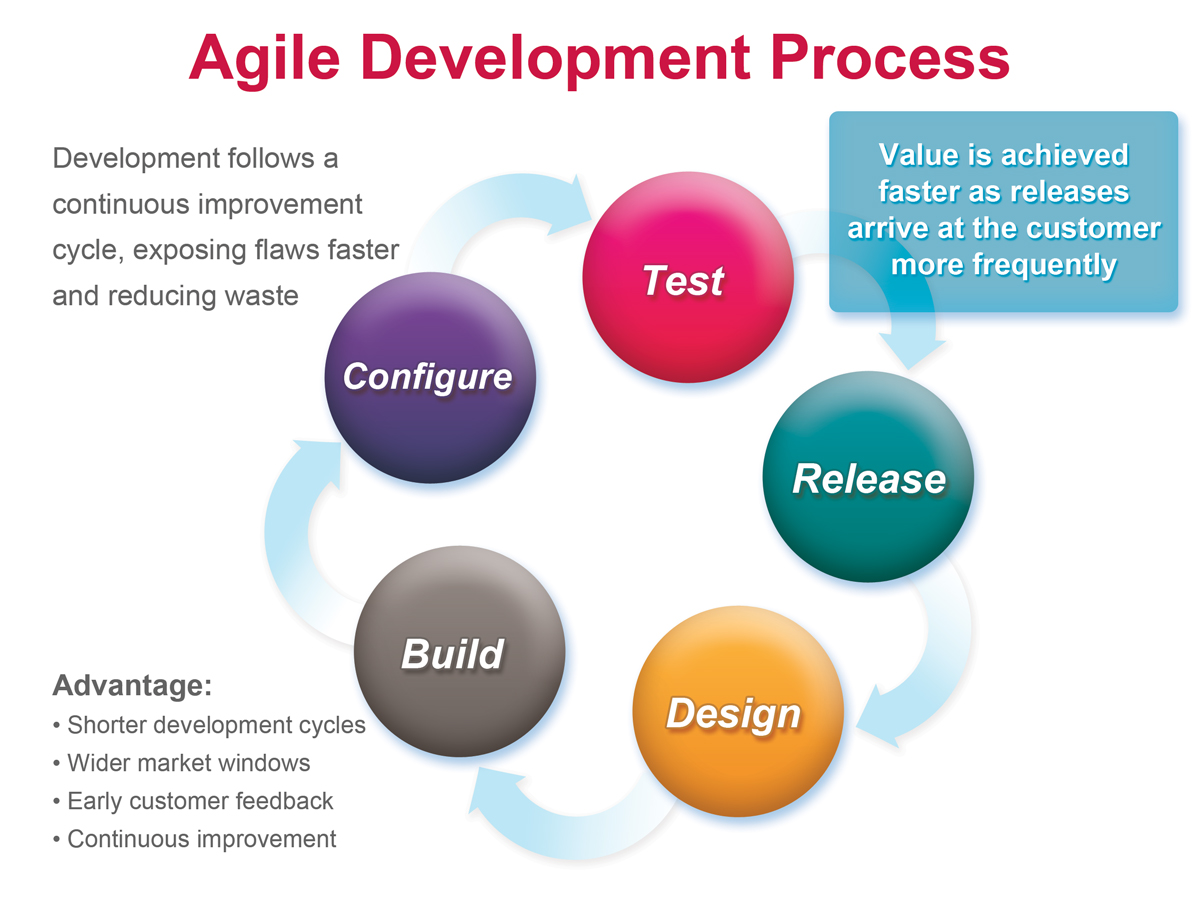
\includegraphics[scale=0.23]{imgs/agiledevelopment.jpg}
\caption{Processo di sviluppo agile\label{agiledevelopment}} 
\end{center}
\end{figure}

La gran parte dei metodi agili tenta di ridurre il rischio di fallimento sia in termini economici, poiché si ha la possibilità di stabilire un tetto di spese limitate che è negoziato frequentemente e monitorato su base costante, sia inteso come forte riduzione del rischio che il cliente si ritrovi in mano funzionalità che non utilizzerà mai o molto raramente. Tutto ciò si può ottenere sviluppando il software in finestre di tempo limitate chiamate \textit{iterazioni} che, in genere, durano qualche settimana.
I fondamenti dei processi agili sono i seguenti:
\begin{itemize}
\item \textbf{iteratività}: prescrive che il processo di sviluppo debba essere ciclico, in modo che le varie fasi siano ripetute più volte in momenti temporali diversi. Questo permette di gestire in modo agile i cambiamenti delle specifiche durante il processo, e non costringe ad aspettare il rilascio del prodotto per poi intraprendere subito una fase di manutenzione, come invece accade con i metodi tradizionali;
\item \textbf{incrementalità}: è il continuo rilascio di versioni parziali del prodotto, le quali inglobano modifiche ed aggiornamenti risultati come necessari alle fasi precedenti. Questo meccanismo permette di rilevare i feedback del committente durante il processo di sviluppo e di adeguare opportunamente il software. In alcuni casi il software rilasciato nelle fasi intermedie è sottoposto anche agli utenti finali, in modo da coglierne le esigenze;
\item \textbf{auto-organizzazione}: il team è lasciato libero di organizzarsi e di adottare di volta in volta le strategie più opportune. Questo favorisce la creatività degli sviluppatori, stimolandoli a trovare soluzioni innovative ai problemi che si presentano;
\item \textbf{emergenza}: bisogna affrontare difficoltà ed imprevisti quando essi si presentano, senza cercare di predeterminarli o una prevenirli. Il principio tradizionale secondo cui un progetto solido deve tener conto dei possibili sviluppi futuri del software viene sovvertito, con la motivazione che si considera inutile spendere tempo e denaro per cercare di prevedere evoluzioni che potrebbero essere disattese.
\end{itemize}
\section{Scelte progettuali}
\subsection{Piattaforma client}
Nell'ambito della localizzazione, la scelta è caduta sulla tecnologia \textbf{GPS}, poichè:
\begin{itemize}
\item \textbf{impossibilità di utilizzo localizzazione indoor}: date le dimensioni considerevoli del sito archeologico, si è ritenuto improbabile l'installazione di una rete WiFi che coprisse tutta l'area, al fine di localizzare tutti i dispositivi presenti;
\item \textbf{inutilità localizzazione cellulare}: la localizzazione cellulare è soggetta a margini di errore ampi per cui, nell'ambito del caso in questione, in cui vi è la necessità di individuare con margini d'errore ridotti la posizione corretta, risulta inutile;
\item \textbf{elevata precisione}: i margini di errore del GPS sono piuttosto bassi, come trattato nel capitolo \ref{tecnologie}.
\end{itemize}


Nella scelta dell'ecosistema su cui sviluppare e presentare un'applicazione per la visita dei siti culturali, \textbf{Windows Phone OS} è stato preferito agli altri, poichè si è tenuto conto di vari fattori:
\begin{itemize}
\item \textbf{originalità}: nello store di Windows Phone, non si trovano applicazioni simili, per cui essa costituirebbe il primo tentativo di visita assistita dei siti culturali;
\item \textbf{utilizzo dispositivi GPS}: l'utilizzo dei dispositivi GPS è molto semplice grazie alle API messe a disposizione da Microsoft. Inoltre si è tenuto conto del background personale.
\end{itemize}

La scelta di Windows Phone OS come piattaforma ha, inoltre, reso quasi obbligatoria l'adozione delle mappe di Bing Maps, che sono supportate nativamente dalla Windows Phone SDK.

\subsection{Piattaforma server}
Il server ospita un application server ed un DBMS.
Il servizio esposto è un \textbf{servizio WCF} (\emph{\url{http://msdn.microsoft.com/en-us/library/dd456779.aspx}}), sviluppato da Microsoft per il trasporto delle informazioni in ambienti distribuiti.
WCF mette assieme le tecnologie di Web Services, Enterprise Service, Message Queuing, fornendo un modello unificato di programmazione per la realizzazione di applicazioni interoperabili.
WCF facilita molto la creazione di un servizio, dal momento che è possibile crearlo ed esporlo tramite IIS (\emph{\url{http://www.iis.net}}) come web service, utilizzando il paradigma REST.

Per la serializzazione dei dati, si è scelto il formato \textbf{GeoRSS} (\emph{\url{http://georss.org}}), un derivato di XML utilizzato specificamente per esportare informazioni georeferenziate.
Un esempio di documento GeoRSS è riportato in figura \ref{georssimage}.
\begin{figure}[h!]
\lstset{language=MYXML}
\begin{lstlisting}
<?xml version="1.0" encoding="utf-8"?>
<feed xmlns="http://www.w3.org/2005/Atom" 
      xmlns:georss="http://www.georss.org/georss" 
      xmlns:gml="http://www.opengis.net/gml">
   <title>Earthquakes</title>
   <subtitle>International earthquake observation labs</subtitle>
   <link href="http://example.org/"/>
   <updated>2005-12-13T18:30:02Z</updated>
   <author>
      <name>Dr. Thaddeus Remor</name>
      <email>tremor@quakelab.edu</email>
   </author>
   <id>urn:uuid:60a76c80-d399-11d9-b93C-0003939e0af6</id>
   <entry>
      <title>M 3.2, Mona Passage</title>
      <link href="http://example.org/2005/09/09/atom01"/>
      <id>urn:uuid:1225c695-cfb8-4ebb-aaaa-80da344efa6a</id>
      <updated>2005-08-17T07:02:32Z</updated>
      <summary>We just had a big one.</summary>
      <georss:point>45.256 -71.92</georss:point>
      </entry>
</feed>
\end{lstlisting}
\caption{Esempio di documento GeoRSS\label{georssimage}}
\end{figure}

Come DMBS si è scelto Sql Server 2012 (\emph{\url{https://www.microsoft.com/italy/server/sql/default.mspx}}), che gestisce al meglio i dati spaziali e su cui c'è la possibilità di utilizzare il framework \textbf{Entity Framework} (\emph{\url{http://msdn.microsoft.com/en-us/data/ef.aspx}}), fornito da \textit{Visual Studio}, trattata di seguito, che consente di creare oggetti a partire dal modello dei dati, al fine di ottenere un alto livello di astrazione.  

\subsection{Ambiente di sviluppo}
In base alle considerazioni ed alle scelte finora effettuate, l'ambiente di sviluppo sarà costituito come di seguito.

\subsubsection{Sistema operativo}
Il sistema operativo utilizzato è Windows 8 (\emph{\url{http://windows.microsoft.com/it-it/windows-8/}}), attualmente il più recente di casa Microsoft.
La scelta è data dalla sua compatibilità con Visual Studio 2012.

\subsubsection{IDE}
L'IDE di sviluppo, in coerenza con le scelte architetturali finora compiute è \textbf{Microsoft Visual Studio} (\emph{\url{http://www.microsoft.com/visualstudio/ita}}), rappresentata con uno screenshot in figura \ref{vsimage}.
Visual Studio permette lo sviluppo di applicazioni console, siti internet, applicazioni grafiche, applicazioni e servizi web, librerie di classi, servizi Windows in tutti i linguaggi di programmazione supportati dal framework .NET, oltre che in tutti i linguaggi di markup, JavaScript e CSS.

\begin{figure}
\begin{center}

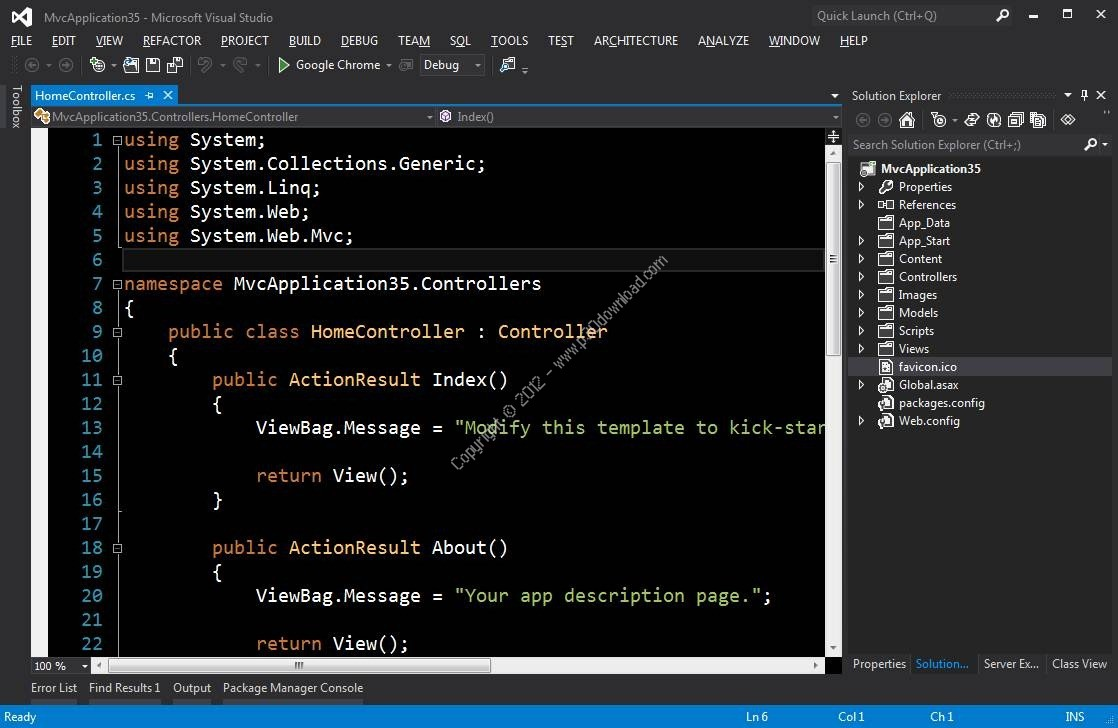
\includegraphics[scale=0.3]{imgs/visualstudio.jpg} 
\caption{Schermata di Visual Studio 2012 Ultimate\label{vsimage}}
\end{center}

\end{figure}
Visual Studio fornisce all’utilizzatore un potente strumento, \textbf{IntelliSense}, che permette
l'autocompletamento del token che il programmatore intende scrivere, oltre che
alla visualizzazione della documentazione e alla gestione delle disambiguità a
video direttamente durante la scrittura del codice.

La versione utilizzata è \textbf{Visual Studio 2012 Ultimate}, lanciata nel settembre 2012.
Essa fornisce numerose nuove features, brevemente elencate:
\begin{itemize}
\item \textbf{Colorazione semantica}: è stata migliorata la colorazione della sintassi, compresi i tipi definiti dall'utente, le macro, i tipi enumerativi e le funzioni;
\item \textbf{Evidenziazione dei riferimenti}: selezione di tutti i riferimenti di un simbolo, una volta selezionato quest'ultimo;
\item \textbf{Nuovo Solution Explorer}: il nuovo Solution Explorer consente agli utenti una visualizzazione per classi o gerarchie di file all'interno del progetto.
E' supportata inoltre la ricerca di chiamate ad una funzione ed utilizzo delle classi;
\item \textbf{Visualizzazione automatica della lista IntelliSense}: IntelliSense è automaticamente visualizzato mentre viene scritto il codice;
\item \textbf{Filtraggio della lista degli elementi}: IntelliSense usa una \textit{fuzzy logic} per determinare quali funzioni/variabili/tipi visualizzare nella lista;
\item \textbf{Code snippets}: è incluso in Intellisense per generare automaticamente frammenti di codice basati sui parametri dell'utente.
\end{itemize}

\subsubsection{Hosting e controllo di versione}
Visual Studio offre, tra i vari servizi, \textbf{Team Foundation Service}, uno strumento di gestione collaborativa del codice che consente di:
\begin{itemize}
\item controllare il proprio codice direttamente in \textit{cloud}, rendendolo accessibile ovunque;
\item gestire il versioning del progetto;
\item gestire la collaborazione nel team;
\item pianificare lo sviluppo agile;
\item gestire il testing e la distribuzione del prodotto.
\end{itemize}



\clearpage{\pagestyle{empty}\cleardoublepage}